\documentclass[12pt,aspectratio=169]{beamer}
\usetheme{metropolis}
\setbeamersize{text margin left=.5cm,text margin right=.5cm}
\usepackage[lf]{carlito}
\usepackage{siunitx}
\usepackage{tikz}
\usepackage{mathpazo}
\usepackage{bm}
\usepackage{mathtools}
\usepackage[ISO]{diffcoeff}
\diffdef{}{ op-symbol=\mathsf{d} }
\usepackage{xcolor,colortbl}

\setmonofont{Ubuntu Mono}
\setlength{\parskip}{0pt}
\renewcommand{\baselinestretch}{1}

\sisetup{
  inter-unit-product=\cdot,
  per-mode=symbol
}

\tikzset{
  >=latex
}

%\newcommand{\iii}{\hat{\bm\imath}}
%\newcommand{\jjj}{\hat{\bm\jmath}}
%\newcommand{\kkk}{\hat{\bm k}}


\title{Class 12: Electrostatics Part 1 (Point Charges)}
\subtitle{Advanced Placement Physics C}
\author[TML]{Dr.\ Timothy Leung}
\institute{Olympiads School}
\date{Updated: Summer 2022}

\newcommand{\pic}[2]{
  \includegraphics[width=#1\textwidth]{#2}
}
\newcommand{\eq}[2]{
  \vspace{#1}{\Large
    \begin{displaymath}
      #2
    \end{displaymath}
  }
}
%\newcommand{\iii}{\ensuremath\hat{\bm{\imath}}}
%\newcommand{\jjj}{\ensuremath\hat{\bm{\jmath}}}
%\newcommand{\kkk}{\ensuremath\hat{\bm{k}}}
\newcommand{\iii}{\ensuremath\hat\imath}
\newcommand{\jjj}{\ensuremath\hat\jmath}
\newcommand{\kkk}{\ensuremath\hat k}



\begin{document}

\begin{frame}
  \maketitle
\end{frame}


\section{Electrostatic Force}

\begin{frame}{Review: The Charges Are}
  We should already know a bit about charge particles:
  \begin{itemize}
  \item A \textbf{proton} carries a \textbf{positive} charge
  \item An \textbf{electron} carries a \textbf{negative} charge
  \item A \emph{net charge} of an object means an excess of protons or electrons
  \item Similar charges are repel; opposite charges attract
  \end{itemize}

  \vspace{.2in}We start with electrostatics:
  \begin{itemize}
  \item Charges that are not moving relative to one another
  \end{itemize}
\end{frame}



\begin{frame}{Coulomb's Law for Electrostatic Force}
  \begin{center}
    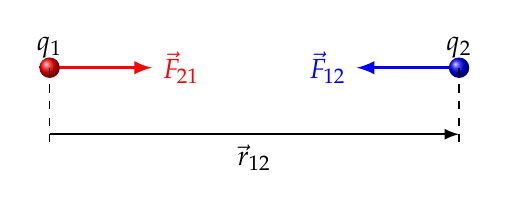
\begin{tikzpicture}[scale=.65]
      \begin{scope}[->,very thick]
        \draw[red] (0,0)--(2,0) node[right]{$\vec F_{21}$};
        \draw[blue](8,0)--(6,0) node[left] {$\vec F_{12}$};
      \end{scope}
      \shade[ball color=red] circle(.2) node[above]{$q_1$};
      \shade[ball color=blue] (8,0) circle(.2) node[above]{$q_2$};
      \draw[dashed] (0,0)--(0,-1.5);
      \draw[dashed] (8,0)--(8,-1.5);
      \draw[->,thick](0,-1.3)--(8,-1.3) node[midway,below]{$\vec r_{12}$};
    \end{tikzpicture}
  \end{center}
  The \textbf{electrostatic force} (or \textbf{coulomb force}) is a mutually
  repulsive/attractive force between all charged objects. The force that charge
  $q_1$ exerts on $q_2$ is given by \textbf{Coulomb's law}:

  \eq{-.2in}{
    \boxed{\vec F_{12}=\frac{kq_1q_2}{|\vec r_{12}|^2}\hat r_{12}}
  }
\end{frame}



\begin{frame}{Coulomb's Law for Electrostatic Force}
  \eq{-.1in}{
    \boxed{\vec F_{12}=\frac{kq_1q_2}{|\vec r_{12}|^2}\hat r_{12}}
  }
  \begin{center}
    \begin{tabular}{l|c|c}
      \rowcolor{pink}
      \textbf{Quantity} & \textbf{Symbol} & \textbf{SI Unit} \\ \hline
      Electrostatic force    & $\vec F_{12}$ & \si\newton \\
      Coulomb's constant     & $k$          & \si{N.m^2/C^2} \\
      Point charges 1 and 2  & $q_1$, $q_2$ &  \si\coulomb \\
      Distance between point charges & $|\vec r_{12}|$ & \si\metre \\
      Unit vector of direction between point charges & $\hat r_{12}$ &
    \end{tabular}
  \end{center}
\end{frame}



\begin{frame}{Coulomb's Constant}

  \eq{-.2in}{
    \boxed{\vec F_{12}=\frac{kq_1q_2}{|\vec r_{12}|^2}\hat r_{12}}
  }

  The constant $k$ in the Coulomb's law is called the
  \textbf{coulomb's constant}, defined as:

  \eq{-.2in}{
    k=\dfrac1{4\pi\epsilon_0}=\SI{8.99e9}{N.m^2/C^2}
  }

  where $\epsilon_0$ is a fundamental constant called the
  \textbf{permittivity of free space}, or \textbf{vacuum permittivity}. It
  measures a vacuum's ability to resist the formation of an electric field:

  \eq{-.2in}{
    \epsilon_0=\SI{8.85e-12}{C^2/N.m^2}
  }
\end{frame}


\begin{frame}{Coulomb's Law for Electrostatic Force}
  \begin{center}
    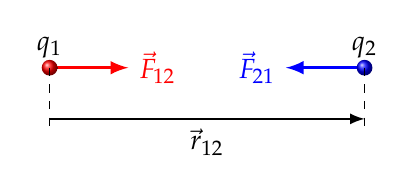
\begin{tikzpicture}[scale=.5]
      \begin{scope}[->,very thick]
        \draw[red] (0,0)--(2,0) node[right]{$\vec F_{12}$};
        \draw[blue](8,0)--(6,0) node[left] {$\vec F_{21}$};
      \end{scope}
      \shade[ball color=red] circle(.2) node[above]{$q_1$};
      \shade[ball color=blue] (8,0) circle(.2) node[above]{$q_2$};
      \draw[dashed] (0,0)--(0,-1.5);
      \draw[dashed] (8,0)--(8,-1.5);
      \draw[->,thick](0,-1.3)--(8,-1.3) node[midway,below]{$\vec r_{12}$};
    \end{tikzpicture}
  \end{center}
  \begin{itemize}
  \item Third law of motion: If $q_1$ exerts an electrostatic force
    $\vec F_{12}$ on $q_2$, then $q_2$ likewise exerts a force of
    $\vec F_{21}=-\vec F_{12}$ on $q_1$. The two forces are equal in magnitude
    and opposite in direction.
  \item $q_1$ and $q_2$ are assumed to be \emph{point charges} that do not
    occupy any space
  \item The scalar form is often used as well, since the direction of $F_q$ can
    easily be found:

    \eq{-.1in}{
      \boxed{F_q=\frac{kq_1q_2}{r^2}}
    }
  \end{itemize}
\end{frame}



\begin{frame}{More Than One Charge}
  \begin{columns}
    \column{.4\textwidth}
    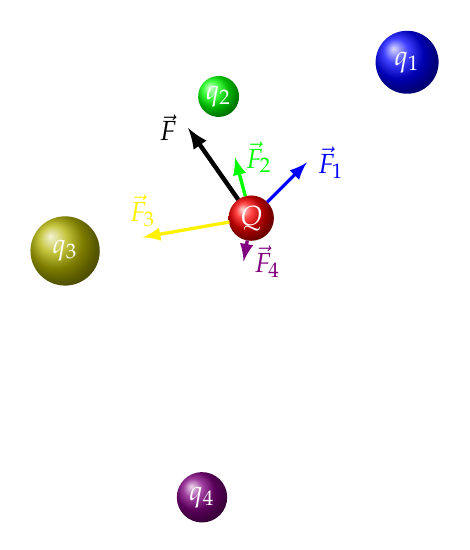
\begin{tikzpicture}[scale=.4]
      \shade[ball color=red] circle(.72) node[white]{$Q$};
      \begin{scope}[rotate=45]
        \draw[->,very thick,blue](.72,0)--(2.5,0) node[right]{$\vec F_1$};
        \shade[ball color=blue] (7,0) circle(1) node[white]{$q_1$};
      \end{scope}
      \uncover<2->{
        \begin{scope}[rotate=105]
          \draw[->,very thick,green](.72,0)--(2,0)
          node[right]{$\vec F_2$};
          \shade[ball color=green] (4,0) circle(.65) node[white]{$q_2$};
        \end{scope}
      }
      \uncover<3->{
        \begin{scope}[rotate=190]
          \draw[->,very thick,yellow](.7,0)--(3.5,0)
          node[above]{$\vec F_3$};
          \shade[ball color=yellow!70!black]
          (6,0) circle(1.1) node[white]{$q_3$};
        \end{scope}
      }
      \uncover<4->{
        \begin{scope}[rotate=260]
          \draw[->,very thick,violet](.72,0)--(1.4,0)
          node[right]{$\vec F_4$};
          \shade[ball color=violet] (9,0) circle(.8) node[white]{$q_4$};
        \end{scope}
      }
      \uncover<5>{
        \begin{scope}[rotate=125]
          \draw[->,ultra thick](.72,0)--(3.5,0) node[left]{$\vec F$};
        \end{scope}
      }
    \end{tikzpicture}

    \column{.6\textwidth}
    For a charge $Q$ that is subjected to the influence of multiple discrete
    point charges $q_i$, the total electrostatic force that $Q$ experiences is
    the vector sum of all the forces $\vec F_i$:
    
    \eq{-.1in}{
      \boxed{\vec F
        =\sum_i\vec F_i
        =kQ\left(\sum_{i=1}^N\frac{q_i}{r_i^2}\hat r_i\right)
      }
    }
  \end{columns}
\end{frame}



\begin{frame}{Continuous Distribution of Charges}
  As $N\rightarrow\infty$, the summation becomes an integral, and can now be
  used to describe the force from charges with \emph{spatial extend} i.e.\
  charges that take up physical space (e.g.\ a continuous distribution of
  charges):

  \eq{-.1in}{
    \boxed{\vec F
      =\int\dl\vec F
      =kQ\int\frac{\dl q}{r^2}\hat r
    }
  }
\end{frame}



\begin{frame}{Infinitesimal Charge $\dl q$}
  The calculation for the infinitesimal charge $\dl q$ is similar to the
  calculation for the infinitesimal mass $\dl m$ earlier in the course (See
  Class 5: Center of Mass)
  \begin{itemize}
  \item Linear charge density (for 1D problems)

    \eq{-.1in}{
      \gamma = \diff qL\quad\rightarrow\quad \dl q =\gamma\dl L
    }

  \item Surface charge density (for 2D problems)

    \eq{-.1in}{
      \sigma=\diff qA\quad\rightarrow\quad \dl q=\sigma\dl A
    }

  \item Charge density (for 3D problems)

    \eq{-.1in}{
      \rho=\diff qV\quad\rightarrow\quad \dl q=\rho\dl V
    }
  \end{itemize}
\end{frame}

    

\section{Electric Field}

\begin{frame}{Electric Field}
  The expression for \textbf{electric field} is obtained by repeating the same
  procedure as with gravitational field, by grouping the variables in
  Coulomb's law:

  \eq{-.1in}{
    F_q
    =\underbrace{
      \left[\frac{kq_1}{|\vec r_{12}|^2}\hat r\right]
    }_{\vec E}q_2
  }

  The electric field $\vec E$ created by $q_1$ is a vector function (called a
  \textbf{vector field}) that shows how it influences other charged particles
  around it.
\end{frame}



\begin{frame}{Electric Field Near a Point Charge}
  The electric field a distance $r$ away from a point charge $q$ is given by:

  \eq{-.1in}{
    \boxed{\vec E(q,\vec r)=\frac{kq}{|\vec r|^2}\hat r}
  }
  \begin{center}
    \begin{tabular}{l|c|c}
      \rowcolor{pink}
      \textbf{Quantity} & \textbf{Symbol} & \textbf{SI Unit} \\ \hline
      Electric field intensity    & $\vec E$ & \si{\newton\per\coulomb}\\
      Coulomb's constant          & $k$   & \si{N.m^2/C^2} \\
      Source charge               & $q$   & \si\coulomb \\
      Distance from source charge & $|\vec r|$   & \si\metre \\
      Outward unit vector from point source & $\hat r$ &
    \end{tabular}
  \end{center}
  The direction of $\vec E$ is radially outward from a positive point charge
  and radially inward toward a negative charge.
\end{frame}



\begin{frame}{More Than One Charge}
  When multiple point charges are present, the total electric field at any
  position $\vec r$ is the vector sum of all the fields $\vec E_i$:
    
  \eq{-.1in}{
    \boxed{\vec E
      =\sum_i\vec E_i
      =k\left(\sum_{i=1}^N\frac{q_i}{r_i^2}\hat r_i\right)
    }
  }
\end{frame}



\begin{frame}{More Than One Charge}
  As $N\rightarrow\infty$, the summation becomes an integral, and can now be
  used to describe the electric field generated by charges with
  \emph{spatial extend}:

  \eq{-.1in}{
    \boxed{
      \vec E=\int\dl\vec E=k\int\frac{\dl q}{r^2}\hat r
    }
  }
  
  This integral may be difficult to compute if the geometry of is complicated,
  but in general, in AP Physics C, there are usually symmetry that can be
  exploited.
\end{frame}



\begin{frame}{Think Electric Field}
  $\vec E$ itself \emph{doesn't do anything} until another charge interacts with
  it. And when there is a charge $q$, the electrostatic force $\vec F_q$ that
  the charge experiences is proportional to $q$ and $\vec E$, regardless of how
  the electric field is generated:

  \eq{-.1in}{
    \boxed{\vec F_q=q\vec E}
  }

  A positive charge in the electric field experiences an electrostatic force
  $\vec F$ in the same direction as $\vec E$.
\end{frame}



\begin{frame}{Electric Field Lines}
  \textbf{Electric field lines} can be used to visualize the direction of the
  electric field.
  \begin{center}
    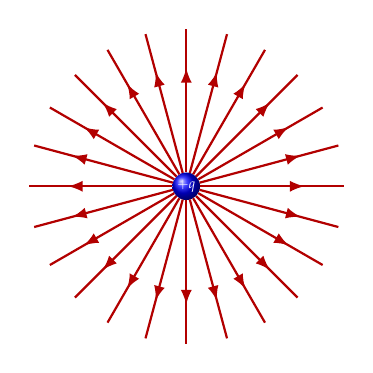
\begin{tikzpicture}[scale=.5]
      \shade[ball color=blue] circle(.35) node[white]{\tiny $+q$};
      \foreach \theta in {15,30,...,360}{
        \begin{scope}[rotate=\theta,red!70!black,thick]
          \draw[->](.35,0)--(3,0);
          \draw (2.8,0)--(4,0);
        \end{scope}
        }
    \end{tikzpicture}
    \hspace{.2in}
    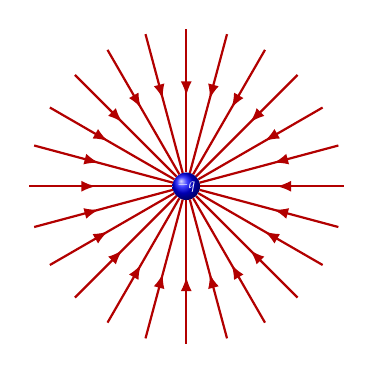
\begin{tikzpicture}[scale=.5]
      \shade[ball color=blue] circle(.35) node[white]{\tiny $-q$};
      \foreach \theta in {15,30,...,360}{
        \begin{scope}[rotate=\theta,red!70!black,thick]
          \draw (.35,0)--(2.5,0);
          \draw[<-](2.3,0)--(4,0);
        \end{scope}
        }
    \end{tikzpicture}
  \end{center}
\end{frame}



\begin{frame}{Electric Field from Multiple Charges}
  \begin{center}
    \pic{.8}{field-lines}
  \end{center}
  \begin{itemize}
  \item Electric field lines must begin and/or end at a charge
  \item Field lines do not cross
  \item Direction of the electric field is tangent to the field lines
  \end{itemize}
\end{frame}



\begin{frame}{Lord of the Ring Charge}
  Suppose you have been given \emph{The One Ring To Rule Them All}, and you
  found out that it is charged! What is its electric field at point $P$ along
  its axis?
  \begin{center}
    \pic{.5}{physicsbook_emism_graphik_35}
  \end{center}
  Note that calculating the electric field away from the axis is very
  difficult.
\end{frame}



\begin{frame}{Electric Field Along Axis of a Ring Charge}
  \begin{columns}
    \column{.3\textwidth}
    \vspace{.1in}
    \pic{1.1}{Fig25}

    \column{.7\textwidth}
    \begin{itemize}
    \item We can separate the electric field $\dl\vec E$ (generated by charge
      $\dl q$) into axial ($\dl E_x$) and radial ($\dl E_\perp$) components
    \item Based on symmetry, $\dl E_\perp$ doesn't contribute to anything; but
      $\dl E_x$ is pretty easy to find:

      \eq{-.2in}{
        \dl E_x =\frac{k\dl q}{r^2}{\color{red}\cos\theta}
        =\frac{k\dl q}{r^2}{\color{red}\frac xr}
        =\frac{kx\dl q}{(x^2+a^2)^{3/2}}
      }
    \end{itemize}
  \end{columns}

  \vspace{.1in}Integrating this over all charges $\dl q$, we have:
  
  \eq{-.1in}{
    E_x =\frac{kx}{(x^2+a^2)^{3/2}}\int \dl q=\boxed{\frac{kQx}{(x^2+a^2)^{3/2}}}
  }
\end{frame}



\begin{frame}{Electric Field Along Axis of a Uniformly Charged Disk}
  Let's extend what we know to a disk of radius $a$ and charge density $\sigma$

  \vspace{.1in}
  \begin{columns}
    \column{.37\textwidth}
    \pic{1}{serway}

    \column{.63\textwidth}
    We start with the solution from the ring problem, and replace $Q$ with
    $\dl q=2\pi\sigma r\dl r$:

    \eq{-.1in}{
      \dl E_x =\frac{2\pi kr\sigma x}{(x^2+r^2)^{3/2}}\dl r
    }

    Integrating over the entire disk:

    \eq{-.1in}{
      E_x =\pi kx\sigma\int_0^a\frac{2r}{(x^2+r^2)^{3/2}}\dl r
    }
    
    This is not an easy integral!
  \end{columns}
\end{frame}



\begin{frame}{Eclectic Field Along Axis of a Uniformly Charged Disk}
  \begin{columns}
    \column{.35\textwidth}
    \pic1{serway}
    
    \column{.65\textwidth}
    Luckily for us, the integral is in the form of $\int u^ndu$,
    with $u=x^2+r^2$ and $n=\frac{-3}2$. You can find the integral in any math
    textbook:

    \eq{-.1in}{
      E_x =2\pi k\sigma\left(1-\frac x{\sqrt{x^2+a^2}}\right)
    }
  \end{columns}
\end{frame}



\section{Electric Potential Energy}

\begin{frame}{Electric Potential Energy}
  The electrostsatic force is a conservative force, therefore the work done
  by $F_q$ is related to the \textbf{electric potential energy} $U_q$:
  
  \eq{-.1in}{
    W=\int\vec F_q\cdot\dl\vec r
    =kq_1q_2\int_{r_1}^{r_2}\frac{\dl r}{r^2}
    =-\frac{kq_1q_2} r\Big|^{r_2}_{r_1}=-\Delta U_q
  }

  where
    
  \eq{-.1in}{
    \boxed{U_q=\frac{kq_1q_2} r}
  }
  \begin{itemize}
  \item $U_q$ can be ($+$) or ($-$), because charges can be either ($+$) or
    ($-$)
  \item Positive work done by $F_q$ decreases $U_q$, while
  \item Negative work done by $F_q$ increases $U_q$
  \item $W$ depends on $r_1$ and $r_2$ but not \emph{how} the charge moves from
    $r_1\rightarrow r_2$
  \end{itemize}
\end{frame}



\begin{frame}{How it Differs from Gravitational Potential Energy}
  \begin{columns}
    \column{.33\textwidth}
    \centering
    Two positive charges:

    \eq{-.3in}{U_q>0}
    
    \column{.33\textwidth}
    \centering
    Two negative charges:

    \eq{-.3in}{U_q>0}
    
    \column{.34\textwidth}
    \centering
    One positive and one negative charge:

    \eq{-.5in}{U_q<0}
  \end{columns}
  \begin{itemize}
  \item $U_q>0$ means positive work is done to bring two charges together from
   $r=\infty$ to $r$ (both charges of the same sign)
  \item $U_q<0$ means negative work (the charges are opposite signs)
  \item For gravitational potential $U_g$ is always $<0$
  \end{itemize}
\end{frame}



\begin{frame}{Relating $U_q$ to $\vec F_q$}
  From the fundamental theorem calculus, we can relate electrostatic force
  ($\vec F_q$) to electric potential energy ($U_q$) by the gradient operator:

  \eq{-.1in}{
    \Delta U_q=-\int\vec F_q\cdot\dl\vec r\quad\rightarrow\quad
    \vec F_q(r)=-\nabla U_q=-\diffp{U_q}r\hat r
  }

  Electrostatic force $\vec F_q$ always points from high to low potential
  energy (steepest descent direction)
\end{frame}



\section{Electric Potential}

\begin{frame}{Electric Potential: Using Gravity as Example}
  An object at a specific location inside a gravitational field has a
  gravitational potential energy proportional to its mass, i.e.\

  \eq{-.1in}{
    U_g=V_gm
  }
  
  This ``constant'' $V_g$ is called the \textbf{gravitational potential}, which
  is the \emph{gravitational potential energy per unit mass}. In the trivial
  case with a uniform gravitational field:

  \eq{-.1in}{
    V_g=\frac{U_g}m=gh
  }

  This also applies to the general case of the gravitational
  potential energy:
  
  \eq{-.1in}{
    V_g=\frac{U_g}m=-\frac{Gm}r
  }  
\end{frame}



\begin{frame}{Electric Potential}
  This is also true for moving a charged particle $q$ against an electric
  electric field created by $q_s$, and the ``constant'' is called the
  \textbf{electric potential}. The unit for electric potential is a \emph{volt}
  which is \emph{one joule per coulomb}, i.e.\
  $\SI1\volt=\SI1{\joule\per\coulomb}$

  \eq{-.1in}{
    \boxed{
      V=\frac{U_q}q
    }
  }

  The electric potential from a source point charge $q_s$ is therefore:

  \eq{-.1in}{
    \boxed{
      V=\frac{kq_s}r
    }
  }
\end{frame}



\begin{frame}{Electric Potential}
  \begin{columns}
    \column{.4\textwidth}
    \centering
    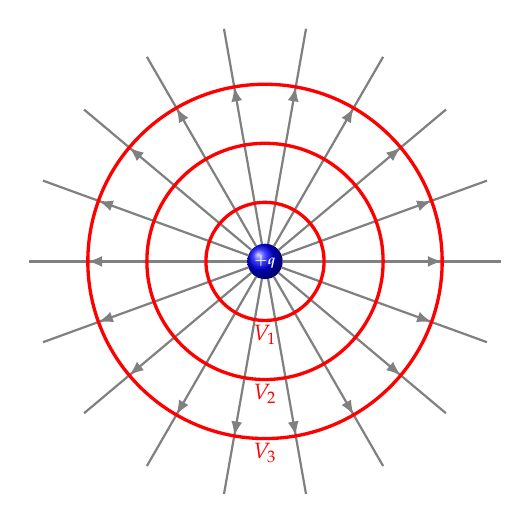
\begin{tikzpicture}[scale=.75]
      \shade[ball color=blue] circle(.3) node[white]{\tiny$\bm{+q}$};
      \foreach \theta in {20,40,...,360}{
        \draw[rotate=\theta,->,gray,thick](.3,0)--(3,0);
        \draw[rotate=\theta,gray,thick](2.8,0)--(4,0);
      }
      \foreach \r in {1,2,3}{
        \draw[very thick,red] circle(\r);
        \node[red,below] at (0,-\r+.09){\footnotesize $V_\r$};
      }
    \end{tikzpicture}
 
    \column{.6\textwidth}
    For a point charge $q$, every point at a distance $r$ will have the same
    electric potential $V(r)$.
    \begin{itemize}
    \item The red lines have the same electric potential; they are called
      \textbf{equipotential lines}, or \textbf{equipotential contours}
    \item Equipotential lines are perpendicular to the electric field lines
    \item Electric field lines always points from higher $V$ toward lower $V$,
      i.e.

      \eq{-.1in}{
        V_1>V_2>V_3
      }
    \end{itemize}
  \end{columns}
\end{frame}



\begin{frame}{Electric Potential}
  \begin{columns}
    \column{.4\textwidth}
    \centering
    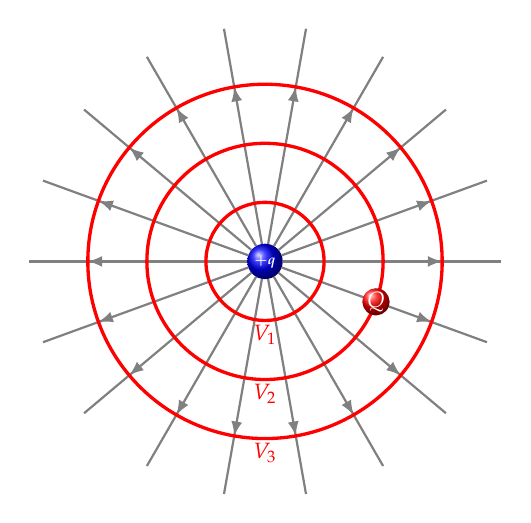
\begin{tikzpicture}[scale=.75]
      \shade[ball color=blue] circle(.3) node[white]{\tiny$\bm{+q}$};
      \foreach \theta in {20,40,...,360}{
        \draw[rotate=\theta,->,gray,thick](.3,0)--(3,0);
        \draw[rotate=\theta,gray,thick](2.8,0)--(4,0);
      }
      \foreach \r in {1,2,3}{
        \draw[very thick,red] circle(\r);
        \node[red,below] at (0,-\r+0.09){\footnotesize$V_\r$};
      }
      \shade[ball color=red,rotate=-20](2,0) circle(.23)
      node[white]{\footnotesize$Q$};
    \end{tikzpicture}
    
    \column{.6\textwidth}
    A charge $Q$ that is placed inside this electric field will now have an
    electric potential energy of:

    \eq{-.1in}{
      U_q=QV=Q\left[\frac{kq}r\right]
    }

    in agreement with equation for electric potential energy
  \end{columns}
\end{frame}



\begin{frame}{Electric Potential from Multiple Charges}
  When there are multiple points charges present, the electric potential is
  given by the summation:

  \eq{-.1in}{
    \boxed{
      V =\underbrace{\frac1{4\pi\epsilon_0}}_k\sum_{i=1}^N\frac{q_i}{r_i}
    }
  }

  As $N\rightarrow\infty$ the summation becomes an integral:

  \eq{-.1in}{
    \boxed{
      V =\frac1{4\pi\epsilon_0}\int\frac{\dl q}r
    }
  }

  where $r$ is the distance to the infinitesimal charge $\dl q$
\end{frame}



\section{Electric Potential Difference}

\begin{frame}{Potential Difference}
  \begin{columns}
    \column{.45\textwidth}
    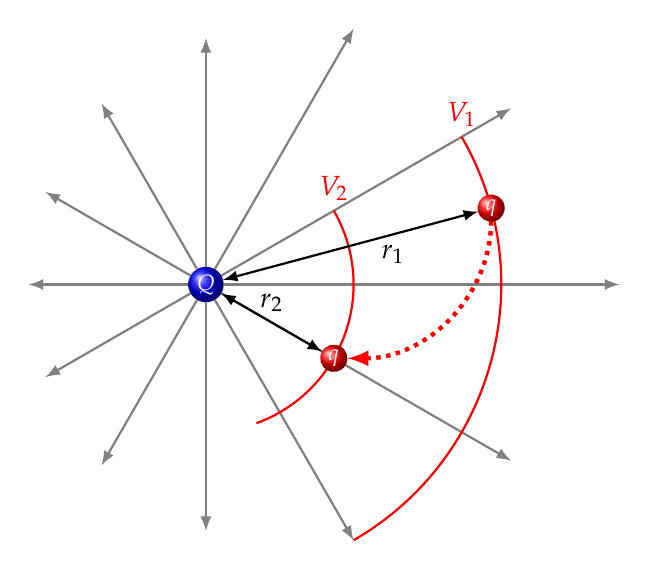
\begin{tikzpicture}[scale=.75]
      \shade[ball color=blue] circle(.3) node[white]{\footnotesize$Q$};
      \foreach \theta in {30,60,...,360}{
        \draw[rotate=\theta,->,gray,thick](.3,0)--({7-4*sin(\theta/2)},0);
      }
      \draw[red,ultra thick,dotted,<-]
      (2.5*cos{30}+.23,-2.5*sin{30}) to[out=0,in=270](5*cos{15},5*sin{15}-.2);
      \draw[thick,red,rotate=-70] (2.5,0) arc(0:100:2.5) node[above]{$V_2$};
      \draw[thick,red,rotate=-60] (5,0)   arc(0:90:5)    node[above]{$V_1$};
      \begin{scope}[rotate=-30]
        \shade[ball color=red](2.5,0) circle(.23) node[white]{\footnotesize$q$};
        \draw[<->,thick](.3,0)--(2.27,0) node[midway,above]{$r_2$};
      \end{scope}
      \begin{scope}[rotate=15]
        \shade[ball color=red](5,0) circle(.23) node[white]{\footnotesize$q$};
        \draw[<->,thick](.3,0)--(4.77,0) node[pos=2/3,below]{$r_1$};
      \end{scope}
    \end{tikzpicture}

    \column{.55\textwidth}
    When a charge is moved from $r_1$ to $r_2$, the change in electric potential
    energy is related to the change in electric potential by:

    \eq{-.1in}{
      \Delta U_q=U_2-U_1=q\Delta V
    }

    where $\Delta V$ is called the \textbf{potential difference}
  \end{columns}
\end{frame}



\begin{frame}{Potential Difference (Voltage)}

  The change in electric potential is called the
  \textbf{electric potential difference} or \textbf{voltage}:

  \eq{-.1in}{
    \boxed{\Delta V=\frac{\Delta U_q}q}\quad\textsf{\normalsize and}\quad
    \boxed{\dl V=\frac{\dl U_q}q}
  }

  Here, we can relate $\Delta V$ to an equation that we knew from Grade 11
  Physics and AP Physics 1/2, which related to the energy dissipated in a
  resistor in a circuit $\Delta U$ to the voltage drop $\Delta V$:
    
  \eq{-.1in}{
    \boxed{\Delta U_q=q\Delta V}
  }

  Electric potential difference also has the unit \emph{volts} (\si\volt)
\end{frame}



\begin{frame}{Relating $V$ to $\vec E$}
  In the same way that the fundamental theorem of calculus relates the 
  electrostatic force ($\vec F_q$) and electric potential energy ($U_q$) by the
  gradient operator, electric field ($\vec E$) and electric potential ($V$) are
  also related the same way:

  \eq{-.1in}{
    \Delta V_q=-\int\vec E_q\cdot\dl\vec r\quad\rightarrow\quad
    \vec E(r)=-\nabla V_q=-\diffp Vr\hat r
  }
  \begin{itemize}
  \item Electrostatic field $\vec E$ always points from high to low electric
    potential
  \item Electric field is also called ``potential gradient''
  \end{itemize}
\end{frame}




\begin{frame}{Getting Those Names Right}
  Remember that these three scalar quantities, as opposed to electrostatic
  force $\vec F_q$ and electric field $\vec E$ which are vectors
  \begin{itemize}
  \item Electric potential energy:
    
    \eq{-.1in}{
      U_q=\frac{kq_1q_2}r
    }
  \item Electric potential:

    \eq{-.1in}{
      V=\frac{U_q}q
    }
  \item Electric potential difference (voltage):

    \eq{-.1in}{
      \Delta V=\frac{\Delta U_q}q
    }
  \end{itemize}
\end{frame}



%\begin{frame}{Relating $U_q$, $V$, $\vec F_q$ and $\vec E$}
%  From the fundamental theorem calculus, we can relate electrostatic force
%  ($\vec F_q$) to electric potential energy ($U_q$) by the gradient operator,
%  and electric field ($\vec E$) to the electric potential ($V$) the same way:
%
%  \eq{-.2in}{
%    \vec F_q(r)=-\nabla U_q=-\diffp{U_q}r\hat r
%    \quad\;\;
%    \vec E(r)=-\nabla V=-\diffp Vr\hat r
%  }
%  \begin{itemize}  
%  \item Electrostatic force $\vec F_q$ always points from high to low potential
%    energy (steepest descent direction)
%  \item Electric field can also be expressed as the change of electric
%    potential per unit distance, which has the unit
%    
%    \eq{-.2in}{
%      \SI1{\newton\per\coulomb}=\SI1{\volt\per\metre}
%    }
%  \item Electric field is also called ``potential gradient''
%  \end{itemize}
%\end{frame}



%\begin{frame}{Equipotential Lines}
%  \begin{center}
%    \pic{.65}{plate3}
%  \end{center}
%  The dotted blue lines are called \textbf{equipotential lines}. They are
%  always \emph{perpendicular} to the electric field lines. Charges moving in
%  the direction of the equipotential lines have constant electric potential
%\end{frame}
\end{document}
